\section{Burst Sequence Optimization}
\label{sec:trng-optimization}

\subsection{Codeword-Level Entropy Isolation}
With knowledge of the ECC, it is possible to construct write sequences
whose codeword-level switching composition is fully controlled. The
all-zeros codeword $\mathbf{0}$ is valid in any linear block code, since
the code forms a vector subspace. A transition from $\mathbf{0}$ to any
other valid codeword is therefore logically unipolar, biasing the device
in one voltage polarity. A transition back to $\mathbf{0}$ is unipolar
in the opposing polarity. This property enables the construction of
fixed-composition write sequences that isolate SET and RESET switching
dynamics. Without ECC knowledge, the only guaranteed method to obtain
latency measurements with identical switching characteristics is to
select a random dataword $u$ producing an unknown codeword $c_?$ and
write the sequence $c_? \to \mathbf{0} \to c_?$. This approach
asymmetrically stresses bitcells and conflates stochastic device
variation with deterministic ECC structure. With ECC knowledge,
wear-leveled sequences that cover all bits within a word can be
constructed and committed to the device in bursts, aggregating many
entropic events per latency measurement.

\subsection{Wear-Leveled Codeword Families}
Three codeword families are constructed for entropy characterization,
each composed of fixed-weight transitions with uniform per-bit switching
counts across the sequence.

\paragraph{Minimum-distance sequence.}
Given an $[n, k, d_{\min}]$ linear code with generator matrix $G$, let
$\mathcal{C}$ denote the set of all minimum-weight codewords:
\begin{equation}
	\mathcal{C} = \{\mathbf{u}G \bmod 2 : \mathrm{wt}(\mathbf{u}G) = d_{\min}\}.
\end{equation}
Because $|\mathcal{C}|$ is small for both devices, it is enumerated
exhaustively. An integer linear program assigns each codeword a
repetition count to minimize the spread in per-bit toggle counts across
the sequence, yielding a provably wear-leveled sequence $S_{d_{\min}}$.

\paragraph{Half-weight sequence.}
For codewords with weight $\lfloor n/2 \rfloor$ or $\lceil n/2 \rceil$,
exhaustive enumeration is intractable. A pool of valid codewords is
generated via SAT construction and codewords are appended greedily, each
step selecting the candidate that minimizes the running spread in
per-bit toggle counts.

\begin{figure}[t!]
	\centering
	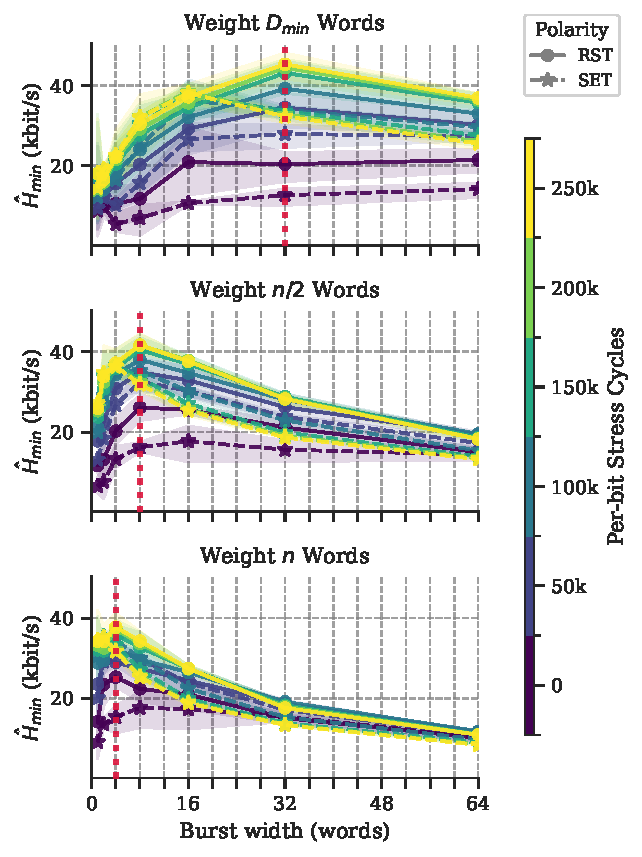
\includegraphics[width=0.49\linewidth]{img/0b_hrate_vs_bw_8m.pdf}
	\hfill
	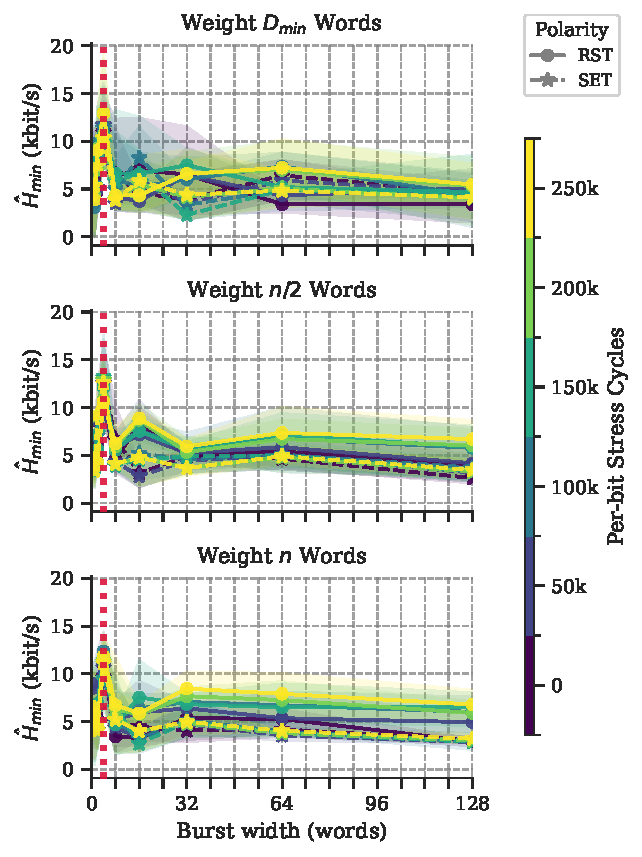
\includegraphics[width=0.50\linewidth]{img/0b_hrate_vs_bw_4m.pdf}
	\caption{
		The entropy rate measured over various wear-leveled codeword sequence compositions and burst sizes for 3  MB85AS4MT 4Mb (right) and 3 MB85AS8MT 8Mb (left) modules from Ramxeed under varying stress levels.
		Each codeword composition is defined by the number of active transitioning bits.
		Several passes are conducted with a uniform stress sequence conducted after each measurement period.
		For the 8M peaks in entropy efficiency are distinguishable at at burst length 32, 8, and 4, for $D_{min}$, $n//2$, and $n$ weight codewords, respectively.
		For the 4M peaks in entropy efficiency are distinguishable at at burst length 4, for $D_{min}$, $n//2$, and $n$ weight codewords.
		\label{fig:opt-burst8m}
	}
\end{figure}

\paragraph{Full-turnover sequence.}
A single all-toggle codeword of weight $n$ is repeated for the required
number of writes. No solver is needed as the existence of the all-ones
codeword $\mathbf{1}$ is trivially verified in any linear block code.

A burst of width $w$ writes $w$ consecutive codeword-sized words in a
single 256\,B SPI transaction. The entropy efficiency per burst is
defined as:
\begin{equation}
	\dot{H}_{\min}(w) = \hat{H}_{\min}(w) / \bar{\tau}_w,
\end{equation}
where $\hat{H}_{\min}(w)$ is the estimated min-entropy per measurement
(bits) for burst width $w$ computed via NIST SP~800-90B, and
$\bar{\tau}_w$ is the mean write latency per codeword within the burst.
This metric captures the trade-off between burst size, entropy yield,
and measurement throughput. The wear-leveling ratio is defined as:
\begin{equation}
	\label{eqn:rt}
	r_t = \frac{n}{r},
\end{equation}
where $r_t < 1$ is the ratio of toggles incurred per write operation
across the entire sequence, $n$ is the codeword length, and $r$ is the
number of parity bits. Figure~\ref{fig:opt-burst8m} shows the entropy efficiency measured across
wear levels and burst widths for the 4M and 8M modules respectively.
Clear peaks in $\dot{H}_{\min}(w)$ are identifiable at burst length 4
for the 4M and at burst lengths 32, 8, and 4 for $D_{\min}$, $n/2$, and
$n$-weight codewords respectively for the 8M. Both devices exhibit
higher RESET $\dot{H}_{\min}$ than SET $\dot{H}_{\min}$, consistent with
the greater cycle-to-cycle variability of SET operations described in
Section~\ref{sec:bg-oxram}. The highest average efficiency across
validated wear levels is achieved with 4-word (32-word) bursts of
weight-$D_{\min}$ codewords on the 4M (8M), achieving 15\,kbits/s
(40.54\,kbits/s).
